\documentclass{article}
\usepackage{graphicx} 
\usepackage{float}
\usepackage{booktabs}
\usepackage{array}
\usepackage{arydshln}
\usepackage{siunitx}
\usepackage{hyperref}
\usepackage{cancel}
\usepackage{changepage}
\usepackage{placeins}
\usepackage{enumitem}
\usepackage{siunitx}
\usepackage{lipsum}
\usepackage[most]{tcolorbox}


%\usepackage{showframe}
\usepackage{times}

\DeclareSIUnit{\atm}{atm}

\usepackage{tabularx}
\usepackage{amsmath, amssymb, amscd, MnSymbol, mathrsfs}
\usepackage{cellspace}
\usepackage{tikz}
\usetikzlibrary{calc,3d, patterns, angles, quotes, decorations.markings, decorations.pathmorphing, hobby}
\usepackage{xfrac}

\usepackage{chemfig}
\usepackage{caption}
\usepackage{bm}
\usepackage{pdfpages}
\usepackage{empheq}
\usepackage{pgfplots}
\usepackage{pgfplotstable}
\usepackage{xstring}

\pgfplotsset{compat=1.18}
\usepackage[oldvoltagedirection]{circuitikz}
\usepackage{microtype}
\usepackage{tikz-3dplot}
\usepackage{textcomp}
% Custom commands
\newcommand{\vect}[1]{\boldsymbol{\mathbf{#1}}}
\newcolumntype{C}{>{\centering\arraybackslash}X}
\newcolumntype{M}[1]{>{\centering\arraybackslash}m{#1}}

%\usetikzlibrary{external}
%\tikzexternalize[prefix=figures/]

\newcommand\myfrac[2]{\sfrac{#1\mkern-1.2mu}{#2}}
\usepackage{xcolor}

% Define custom colors
\definecolor{darkblue}{rgb}{0.1,0.1,0.5} %  dark blue shade
\definecolor{formalshade}{rgb}{0.95,0.95,1} % light blue shade for the background

% For the adjustwidth environment
\PassOptionsToPackage{strict}{changepage}
\usepackage{changepage}

% For formal definitions
\usepackage{framed}

\newcommand{\formalsource}{} % Initialize an empty macro to store the source text

\newenvironment{formal}[3][]{% Start of the environment
	\renewcommand{\formalsource}{#1}% Store the optional argument
	\def\FrameCommand{%
		\hspace{1pt}%
		{\color{#2}\vrule width 2pt}%
		{\color{#3}\vrule width 4pt}%
		\colorbox{#3}%
	}%
	\MakeFramed{\advance\hsize-\width\FrameRestore}%
	\noindent\hspace{-4.55pt}% Disable indenting the first paragraph
	\begin{adjustwidth}{}{7pt}%
		\vspace{2pt}%
	}%
	{%
		\vspace{4pt}%
		\ifx\formalsource\empty % Check if the source is empty
		\else
		\hfill{\footnotesize{\formalsource}}% Align source to the bottom-right
		\fi
	\end{adjustwidth}\endMakeFramed%
}


% Custom itemize list with images for positive and negative items
\newlist{gitemize}{itemize}{1} % Just one level for the list
\setlist[gitemize,1]{
	leftmargin=2.8em, % Adjust the margin for the list
	labelsep=1em % Control the space between the label and the list item
}

% Define checkmark and cross symbols for positive and negative items
\newcommand{\checkitem}{\raisebox{-0.25\height}{\includegraphics[width=0.4cm]{checkmark.png}}}
\newcommand{\crossitem}{\raisebox{-0.25\height}{\includegraphics[width=0.4cm]{cross.png}}}


\usepackage[left=0.8in,right=0.8in,top=0.5in,bottom=0.69in,includeheadfoot,letterpaper]{geometry}
\usepackage{fancyhdr}
\usepackage{graphicx}
\usepackage{tabularray}
\usepackage{varwidth} 


\newcommand{\wm}[2]{%
	\begin{minipage}{#1\textwidth}
		\centering
		#2
	\end{minipage}%
}

\pagestyle{fancy}
\fancyhf{}


\renewcommand{\headrulewidth}{0.4pt}
\renewcommand{\footrulewidth}{0.4pt}

\fancyhead[L]{
\includegraphics[height=1.2cm]{images/Kingston_University_London_logo_200-tablet.png}}
\fancyhead[R]{EG4023 – ME – IMechE Design Challenge Project}
\fancyfoot[C]{Department of Mechanical Engineering}
\fancyfoot[R]{\thepage}

\usepackage{scalerel}
\usepackage{pythonhighlight}
\setlength{\headheight}{30pt}
\setlength{\footskip}{20pt}



\usepackage[export]{adjustbox}
\usepackage{tocloft}
\renewcommand{\cfttoctitlefont}{}
\renewcommand{\contentsname}{}
\renewcommand{\cftsecleader}{\cftdotfill{\cftdotsep}}

\setlength{\cftbeforesecskip}{0.5em}



\usepackage{hyperref}    % For hyperlinks
\usepackage{xurl}        % For better URL handling
\hypersetup{
	colorlinks=true,
	linkcolor=blue!50!black,
	urlcolor=blue,       % Color for URLs
}


\definecolor{ChineseGold}{HTML}{C59401}
\definecolor{AmericanGold}{HTML}{D3AF37}
\definecolor{MetallicSunburst}{HTML}{A77C37}
\definecolor{GoldenBrown}{HTML}{996515}
\definecolor{DarkBrown}{HTML}{674222}
\definecolor{SkyBlue}{HTML}{87CEEB}      % Soft and bright
\definecolor{BabyBlue}{HTML}{89CFF0}     % Gentle, pastel-like
\definecolor{SteelBlue}{HTML}{4682B4}    % Rich but not overpowering
\definecolor{RoyalBlue}{HTML}{4169E1}    % Strong, slightly purplish
\definecolor{MidnightBlue}{HTML}{191970} % Almost black, deep navy
\definecolor{PrussianBlue}{HTML}{003153} % Very deep blue with a classic look
\definecolor{mainblue}{HTML}{1D73BE}

\usepackage{listings}

\definecolor{codegreen}{rgb}{0,0.6,0}
\definecolor{codegray}{rgb}{0.5,0.5,0.5}
\definecolor{codepurple}{rgb}{0.58,0,0.82}
\definecolor{backcolour}{rgb}{0.95,0.95,0.92}

\lstdefinestyle{mystyle}{
	backgroundcolor=\color{white!97!gray},   
	commentstyle=\color{codegreen},
	keywordstyle=\color{purple},
	numberstyle=\tiny\color{codegray},
	stringstyle=\color{orange},
	basicstyle=\ttfamily\scriptsize,
	breakatwhitespace=false,         
	breaklines=true,                 
	captionpos=b,                    
	keepspaces=true,                 
	numbers=left,                    
	numbersep=5pt,                  
	showspaces=false,                
	showstringspaces=false,
	showtabs=false,                  
	tabsize=2
}

\lstset{style=mystyle}

%Refer to the equation as \eqref{equation}.
\usepackage{caption}  % This package allows captioning outside of a float
\usepackage[export]{adjustbox}


\usetikzlibrary{patterns}

\usetikzlibrary{patterns.meta}
\usepackage[para]{footmisc} % Example of making footnotes run together in a paragraph

\definecolor{darkgreen}{rgb}{0.0, 0.5, 0.0}

\usepackage{datetime}

\usepackage{etoolbox}

\makeatletter
\def\tagform@#1{\maketag@@@{{Eq.~#1}}} 
\makeatother

\usepackage{ifthen}
\usepackage{calc}
\usepackage{datenumber}

\usepackage{physics}
\usepackage[outline]{contour}
\usetikzlibrary{patterns,decorations.pathmorphing}
\usetikzlibrary{arrows.meta}
\tikzset{>=latex}
\contourlength{1.1pt}

\colorlet{mydarkblue}{blue!50!black}
\colorlet{myred}{red!65!black}
\colorlet{watercol}{blue!80!cyan!10!white}
\colorlet{darkwatercol}{blue!80!cyan!20!white}
\tikzstyle{piston}=[blue!50!black,top color=blue!30,bottom color=blue!50,middle color=blue!20,shading angle=0]
\tikzstyle{water}=[draw=mydarkblue,top color=watercol!90,bottom color=watercol!90!black,shading angle=5]
\tikzstyle{vertical water}=[water,
top color=watercol!90!black!90,bottom color=watercol!90!black!90,middle color=watercol!80,shading angle=90]
\def\tick#1#2{\draw[thick] (#1)++(#2:0.1) --++ (#2-180:0.2)}



\newcounter{deadlineyear}\setcounter{deadlineyear}{2025}
\newcounter{deadlinemonth}\setcounter{deadlinemonth}{4}
\newcounter{deadlineday}\setcounter{deadlineday}{9}
\newcounter{deadlinetime}\setcounter{deadlinetime}{1439} % Default: 23:59 (1439 minutes)
\newcounter{mydatenumber}
\newcounter{currentdate}
\newcounter{daysdiff}
\newcounter{currenttime}
\newcounter{totalminutes}
\newcounter{displaydays}
\newcounter{remainingmins}
\newcounter{displayhours}
\newcounter{displaymins}

% ====== MACROS ======
% Set deadline time (e.g., \setdeadlinetime{23}{59})
\newcommand{\setdeadlinetime}[2]{%
	\setcounter{deadlinetime}{#1 * 60 + #2}%
}

% Main calculation command
\newcommand{\timeUntilDeadline}{%
	% Calculate days between dates
	\setmydatenumber{mydatenumber}{\thedeadlineyear}{\thedeadlinemonth}{\thedeadlineday}%
	\setmydatenumber{currentdate}{\the\year}{\the\month}{\the\day}%
	\setcounter{daysdiff}{\themydatenumber - \thecurrentdate}%
	
	% Get current time in minutes since midnight
	\setcounter{currenttime}{\time}%
	
	% Calculate total remaining minutes (deadline time - current time)
	\setcounter{totalminutes}{\thedaysdiff * 1440 + \thedeadlinetime - \thecurrenttime}%
	
	% Check deadline status
	\ifnum\thetotalminutes < 0
	\textbf{\color{red}Deadline passed!}%
	\else
	% Calculate time components
	\setcounter{displaydays}{\thetotalminutes / 1440}%
	\setcounter{remainingmins}{\thetotalminutes - \thedisplaydays * 1440}%
	\setcounter{displayhours}{\theremainingmins / 60}%
	\setcounter{displaymins}{\theremainingmins - \thedisplayhours * 60}%
	
	% Format output
	\textbf{%
		\ifnum\thedisplaydays > 0
		\thedisplaydays\ day\ifnum\thedisplaydays > 1 s\fi%
		\ifnum\thedisplayhours > 0
		\ifnum\thedisplaymins > 0, \else\ and \fi%
		\else
		\ifnum\thedisplaymins > 0\ and \fi%
		\fi%
		\fi%
		\ifnum\thedisplayhours > 0
		\thedisplayhours\ hour\ifnum\thedisplayhours > 1 s\fi%
		\ifnum\thedisplaymins > 0\ and \fi%
		\fi%
		\ifnum\thedisplaymins > 0
		\thedisplaymins\ minute\ifnum\thedisplaymins > 1 s\fi%
		\fi%
		\ left%
	}%
	\fi
}

\definecolor{mygreen}{HTML}{07a56d}

\newtcbtheorem{briefillus}{Definiton}{
	enhanced,
	sharp corners,
	attach boxed title to top left={
		xshift=0pt, 
		yshift=-\tcboxedtitleheight, 
		yshifttext=-\tcboxedtitleheight/2-0.5em
	},
	colback=white,
	colframe=black,
	fonttitle=\bfseries,
	coltitle=white,
	boxed title style={
		rounded corners,
		arc=2pt,
		size=small,
		colback=black,
		colframe=black,
	},
	leftrule=0pt, 
	rightrule=0pt, 
}{thm}

\usepackage{titlesec}

\titleformat{\section}[block]{\vspace*{-10pt}\centering\normalfont\Large\bfseries\color{mainblue}}{\color{mainblue}\thesection}{1em}{}
\titleformat{\subsection}[block]{\normalfont\large\bfseries\color{mainblue}}{\color{mainblue}\thesubsection}{1em}{}
\titleformat{\subsubsection}[block]{\normalfont\normalsize\bfseries\color{mainblue}}{\color{mainblue}\thesubsubsection}{1em}{}

\begin{document}

\thispagestyle{empty}

\color{white}
\tikz[remember picture,overlay] \node[opacity=1,inner sep=0pt] at (current page.center){
\includegraphics[width=\paperwidth,height=\paperheight]{images/A4-document-placeholder-medium-blue_0.jpg-ezgif.com-webp-to-jpg-converter(2).jpg}};

\vspace*{\fill}
\begin{center}
	\textbf{\Huge IMechE Design Challenge}\\[10pt]
	\LARGE \textbf{Group Report and Logbook}
\end{center}
\vspace*{\fill}

\Large    
\begin{tabular}{@{}l l l@{}}
	\textbf{Submitted by:}  & Samatar Ahmed (Group Leader) \phantom{ssssssssss}& K2374854\\
	& Sakariye Abiikar & K2371673 \\
	& Jayden Balgobind & K2421484\\
	& Hector Huser & K2367380\\
	& Hashaam Khan & K2371729\\
	& Josh Mossman & K2457119\\
\end{tabular}

\vspace*{\fill}

\begin{tabular}{@{}l l@{}}
	\textbf{Key Dates:} & Date of practical: Thursday 3$^{\text{rd}}$ April, 2025 \\
	& Deadline: Wednesday 9$^{\text{th}}$ April, 2025 23:59\\
	& Last Updated: \today\, \currenttime \\
	& Days left until deadline: \timeUntilDeadline \\
\end{tabular}
\vspace*{\fill}

\large
\newpage\thispagestyle{empty}\newgeometry{top=0.7in,bottom=0.6in,left=0.8in,right=0.8in}
\tikz[remember picture,overlay] \node[opacity=0.5,inner sep=0pt] at (current page.center){
\includegraphics[width=\paperwidth,height=\paperheight]{images/a13d25fa5178ce400e90e65f61d696d3.jpg}};

\color{black}
\vspace*{\fill}
\noindent
\begin{tblr}{
		colspec={Q[5.4cm]Q[5.4cm]Q[5.4cm]},
		hlines,vlines,
		cells={valign=m,halign=c},
		rows={ht=2\baselineskip},
		row{1}={ht=1\baselineskip,font=\bfseries,fg=mainblue!90!white},
	}
	MODULE NO. & MODULE TITLE & MODULE LEADER \\
	EG4023 & Introduction to Engineering Design and Manufacture & Dr Andy Curley \\\hline
	Assignment Title: & \SetCell[c=2]{c} IMechE Design Challenge Project --- Group Report and Logbook &  \\	
\end{tblr}\\[1em]
\begin{tblr}{
		colspec={Q[5.4cm]Q[11.24cm]},
		hlines,vlines,
		cells={valign=m,halign=c},
		rows={ht=2\baselineskip},
	}
	Group Name: & Group 1  \\
\end{tblr}\\[1em]
\begin{minipage}{0.98\textwidth}
	\vspace*{0.1mm}
	\begin{center}
		\fbox{
			\begin{minipage}[c][16cm][c]{\textwidth}
				\centering
				\includegraphics[height=10cm]{example-image}
			\end{minipage}
		}
	\end{center}
	\vspace*{1em}
\end{minipage}
\vspace*{\fill}


\newpage\thispagestyle{empty}

\tikz[remember picture,overlay] \node[opacity=0.5,inner sep=0pt] at (current page.center){
\includegraphics[width=\paperwidth,height=\paperheight]{images/a13d25fa5178ce400e90e65f61d696d3.jpg}};

\noindent\vspace*{4em}

\begin{center}
	\LARGE \textbf{\textcolor{mainblue}{Contribution Table}}\\[2em]
	\large\vspace*{2em}
\begin{tblr}{
		colspec={Q[5cm]Q[5cm]Q[5cm]},
		hlines,vlines,
		cells={valign=m,halign=c},
		rows={ht=4\baselineskip},
		row{1}={ht=1.5\baselineskip,font=\bfseries,fg=mainblue!90!white},
	}
	 Student & Contribution & Picture \\ 
	 Samatar Ahmed &  & 
\includegraphics[width=2cm,valign=c]{images/profile.png} \\ 
	 Sakariye Abiikar &  & 
\includegraphics[width=2cm,valign=c]{images/profile.png} \\ 
	 Jayden Balgobind &  &  
\includegraphics[width=2cm,valign=c]{images/profile.png}\\
	 Hector Huser &  & 
\includegraphics[width=2cm,valign=c]{images/profile.png} \\ 
	 Hashaam Khan &  & 
\includegraphics[width=2cm,valign=c]{images/profile.png}\\
	 Josh Mossman &  & 
\includegraphics[width=2cm,valign=c]{images/profile.png} \\
\end{tblr}
\end{center}	
\vspace*{\fill}

\normalsize
\newpage\newgeometry{top=0.2in,bottom=1in,left=0.8in,right=0.8in}\tikz[remember picture,overlay] \node[opacity=0.5,inner sep=0pt] at (current page.center){
\includegraphics[width=\paperwidth,height=\paperheight]{images/a13d25fa5178ce400e90e65f61d696d3.jpg}};
\noindent\vspace{7em}\pagenumbering{gobble}
\begin{center}
	\LARGE \textbf{\textcolor{mainblue}{Table of Contents}}\\[-7em]
\end{center}
{
	\hypersetup{linkcolor=black}
	\tableofcontents
}    


\large\newpage\restoregeometry
\noindent\pagenumbering{arabic}\setcounter{page}{1}

\section{Abstract}
This report/logbook serves as a comprehensive account of our group's involvement in the IMechE Design Challenge 2025, which tasks first-year engineering students with designing, building, and testing an autonomous robotic charging device. Although the design appeared simple at first, transforming our ideas into a working prototype presented significant challenges. Throughout the project, we encountered technical and mechanical obstacles that required creative problem-solving and adaptation. This report details the design process, challenges faced, solutions implemented, and the collaborative efforts that led to the final product. Through this challenge, we gained invaluable experience in practical engineering, teamwork, and the application of analogue electronics principles, all while exploring the potential of autonomous and sustainable technologies.

\newpage
\section{Introduction}
The \textit{Design Challenge}, organized annually by the Institution of Mechanical Engineers (IMechE), invites first-year undergraduate engineering students to participate in a competition that tests their skills in designing, building, and testing innovative solutions. This year, the challenge involves designing an \textbf{autonomous robotic charging device}. 
\subsection{Competition Overview}
Design a self-contained device that autonomously connects/disconnects from a charging target, simulating EV charging. It must navigate a 1m-wide horizontal track (1.4-4.0m length) to engage a vertical wall (0.3m min height) under these rules:
\subsubsection*{Key Requirements}
\begin{itemize}[itemsep=-0.5mm,topsep=0pt]
	\item Complete mission autonomously within 3 minutes
	\item Tolerate real-world conditions (8mm/1.5m level variance, 3mm surface gaps)
	\item Engage charging target (50mm height for single, 50/150mm for double target)
	\item Maintain contact for specified charging duration
	\item Handle three distance ranges:
	\begin{itemize}[noitemsep,topsep=0pt]
		\item Short: 1.4-2.2m
		\item Medium: 2.4-3.0m
		\item Long: 3.2-4.0m
	\end{itemize}
\end{itemize}
\subsubsection*{Track Specifications}
\begin{itemize}[noitemsep,topsep=0pt]
	\item \textbf{Material}: Commercial wood boards (plywood/OSB/MDF) or approved hard floors
	\item \textbf{Construction}: Joined boards (3mm max level variance, 2mm max gaps)
	\item \textbf{Layout}: Multiple lanes with 1m spacing
\end{itemize}
\begin{center}
	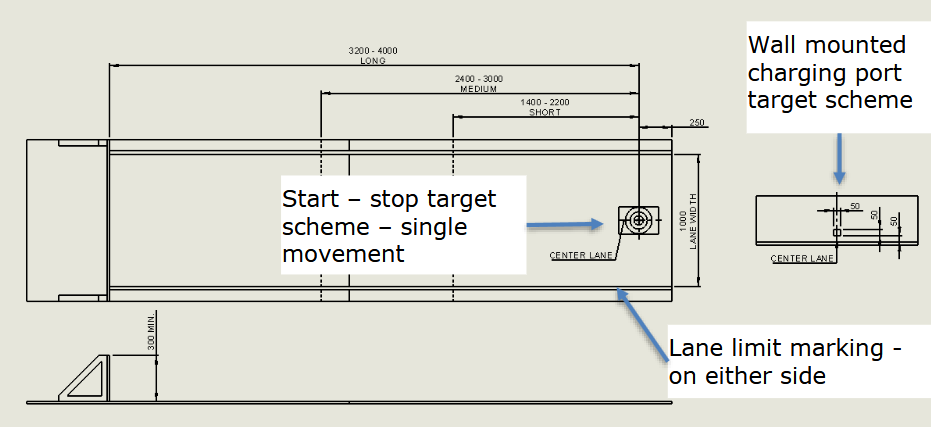
\includegraphics[width=0.8\textwidth]{extracted_images/image_4_2.png}\\
	\small\textbf{Figure 3:} Lane setup (dimensions in mm)
\end{center}
\subsubsection*{Measurement Tolerance}
$\pm$10mm using a single tape measure. Barrier positions vary in 50mm increments within each range.


\section{Product Design Specification}
Info is catered to the Foundation Group.
\subsection{Dimensional Requirements}
\begin{itemize}[itemsep=-0.7mm]
	\item Maximum working envelope: 400mm $\times$ 400mm $\times$ 400mm (including all components)
	\item Must maintain envelope compliance during all competition movements
	\item Front plunger (plug simulator):
	\begin{itemize}[noitemsep,topsep=0pt]
		\item Max dimensions: 10mm $\times$ 10mm
		\item Minimum protrusion: 10mm from device body when disengaged
	\end{itemize}
\end{itemize}

\subsection{Required Components}
\begin{itemize}[itemsep=-0.7mm]
	\item \textbf{Rear datum pointer} (RS Components 397-4954):
	\begin{itemize}[noitemsep,topsep=0pt]
		\item Must remain vertical (pointing downward)
		\item Max 6mm clearance from track surface
		\item Determines device positioning
	\end{itemize}
	\item \textbf{Single front plunger} (non-adjustable height for Foundation Group)
\end{itemize}

\subsection{Visual Indicators}
\begin{itemize}[noitemsep,topsep=0pt]
	\item Continuous green light during operation
	\item Red light + audible signal upon successful wall engagement
\end{itemize}

\subsection{Technical Restrictions}
\begin{itemize}[itemsep=-0.7mm,topsep=0pt]
	\item \textbf{No programmable circuitry} permitted (analog systems only)
	\item All repairs must be completed within allocated competition time
	\item Device must be fully self-contained (no external control)
\end{itemize}

\begin{figure}[h]
	\centering
	\begin{minipage}{0.45\textwidth}
		\centering
		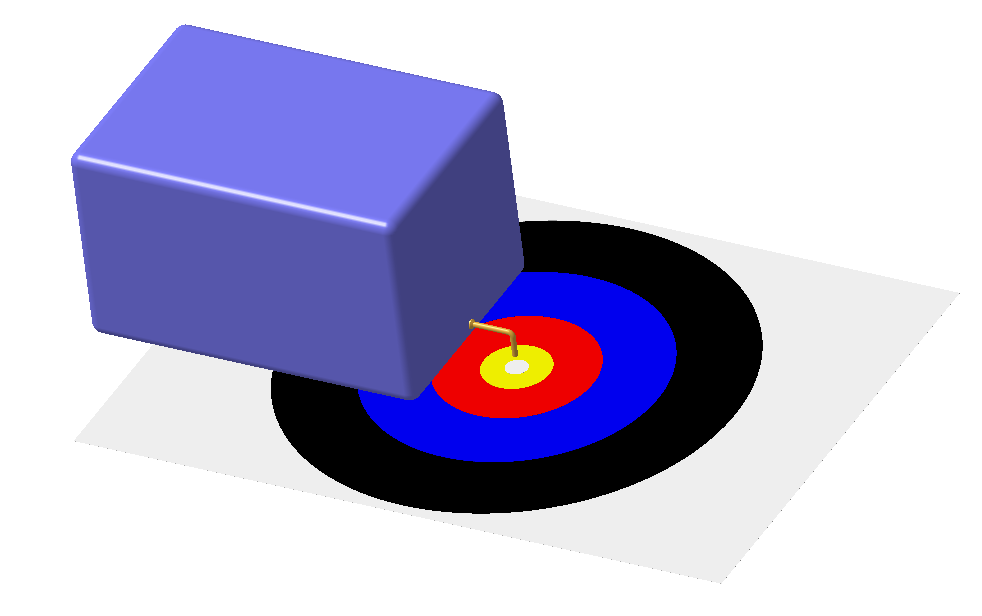
\includegraphics[width=0.8\linewidth]{extracted_images/image_10_2.png}
		\caption{Front plunger requirements}
	\end{minipage}
	\begin{minipage}{0.45\textwidth}
		\centering
		
\includegraphics[width=0.8\textwidth,height=3.2cm]{extracted_images/image_10_1.png}
		\caption{Datum pointer specification}
	\end{minipage}
\end{figure}
\subsection*{Key Differences from Advanced Category}
\begin{itemize}[itemsep=-0.7mm]
	\item No height adjustment capability required
	\item No programming or digital components allowed
	\item Simplified single-target operation
\end{itemize}


\newpage\newgeometry{left=0.8in,right=0.8in,top=1in,bottom=0.5in}
\section{Design Concepts}

\begin{minipage}{0.59\textwidth}
\subsection{Design Concept 1}
This was our initial concept idea, which had the advantage of being simple with minimal refinement. However, its main drawback was the high cost. While the model was accurate and met the specifications, its complexity and expensive manufacturing process made it difficult to produce.\\[8pt]
A major issue with this design is that high manufacturing costs can make large-scale production unfeasible. When a product is too costly to produce, it affects everything, from labor and machinery costs to production time, resulting in increased expenses and longer production timelines.
\end{minipage}\hfill
\begin{minipage}{0.4\textwidth}
\centering
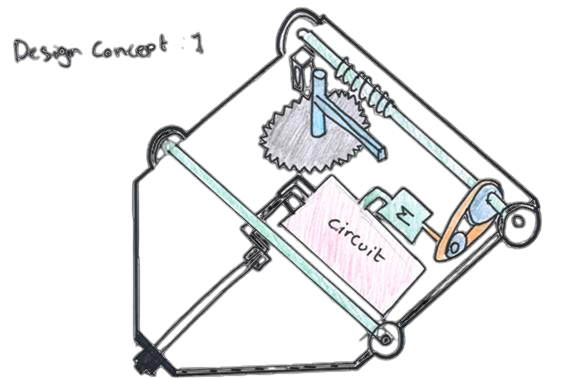
\includegraphics[width=1\textwidth]{images/image_6_2-Photoroom.png}
\captionof{figure}{Design Concept 1}
\end{minipage}\\[8pt]
The positives of this design is that it does meet the required specifications as it does fit the purpose of its role.\\[1em]
\begin{minipage}{0.59\textwidth}
	\subsection{Design Concept 2}
	This was our second design, which was simple and aesthetically pleasing. Its major strength was its ease of construction and compact size, which provided extra space for potential part exchanges or swaps. It was an adaptable design, but the main drawback was its susceptibility to breakages.\\[8pt]
	The negatives of this build are that it is prone to breakages, making it unreliable. This is crucial because during the testing phase, the design must pass to function correctly. If it is prone to breaking easily, it will reduce its longevity as materials deteriorate over time. The small size also means less room for improvements if needed.
\end{minipage}\hfill
\begin{minipage}{0.35\textwidth}
	\centering
	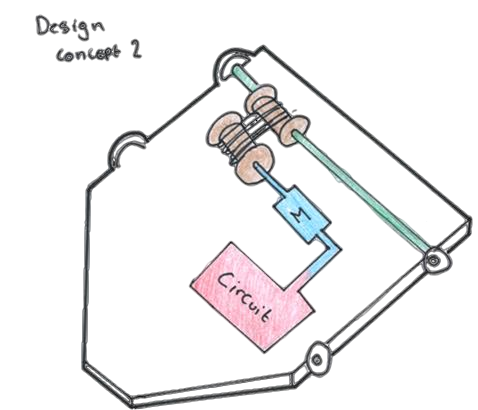
\includegraphics[width=1\textwidth]{images/image_7_2-Photoroom.png}
	\captionof{figure}{Design Concept 2}
\end{minipage}\\[4pt]
However, it is an aesthetic and versatile design, easy to swap parts if it breaks. The compactness is efficient for aerodynamics, and the lightness comes from the absence of bulky components.\\[1em]
\begin{minipage}{0.59\textwidth}
	\subsection{Design Concept 3}
	This was our final concept idea, which, like the first, had minimal refinement. Its major drawback was the cost, as it involved many unique moving parts. Although this design was durable and strong, it exceeded the budget outlined in the technical specifications.\\[8pt]
	The overall budget of this design was very high due to the numerous parts required, which increased manufacturing costs. There was also a lack of refinement, leading to inefficiencies in the design itself. The complexity of the build made assembly difficult, resulting in a higher likelihood of errors that could have been easily fixed with a simpler design. 
\end{minipage}\hfill
\begin{minipage}{0.4\textwidth}
	\centering
	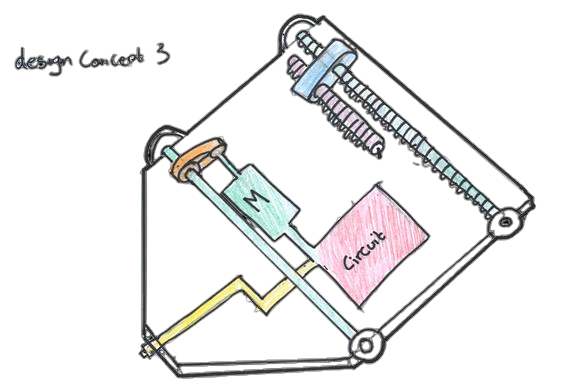
\includegraphics[width=1\textwidth]{images/image_8_2-Photoroom.png}
	\captionof{figure}{Design Concept 3}
\end{minipage}\\[8pt]
Despite this, it was a durable and strong design that could withstand impact and perform well.

\newpage\restoregeometry
\section{CAD}


\newpage
\section{Electronics}
Oh yes

\newpage

\section{BOM (Bill of materials)}
Parts listed for the device are stated below. Every part that was mentioned was used within the final design of the device.
\begin{itemize}[itemsep=-1mm]
	\item Wheels x 4
	\item Lead thread hub x 4
	\item Base x 1
	\item Screw and lead x 1
	\item Plastic tube x 1
	\item Thread screw x 1
	\item Motor x 1
	\item Datum x 1
	\item Belt x 1
\end{itemize}\noindent
Below is a list of the electrical components that were used within the device. Everything mentioned below was used in the final design of the device.
\begin{itemize}[itemsep=-1mm]
	\item 9V Battery
	\item 555 Timer
	\item 10 k$\Omega$ Resistor
	\item 1 k$\Omega$ Resistor
	\item 2.2$\sim\mu$F Capacitor
	\item Red LED
	\item Green LED
	\item 470$\sim\mu$F Capacitor
	\item DPDT Switch
\end{itemize}
These were parts that were essential when building the device. Since we used all components, we did not waste any money, which could have impacted our costs — we could have used the money to purchase better equipment or parts if needed.

\newpage
\section{Manufacturing process}


\newpage
\section{Final design}
\begin{center}
	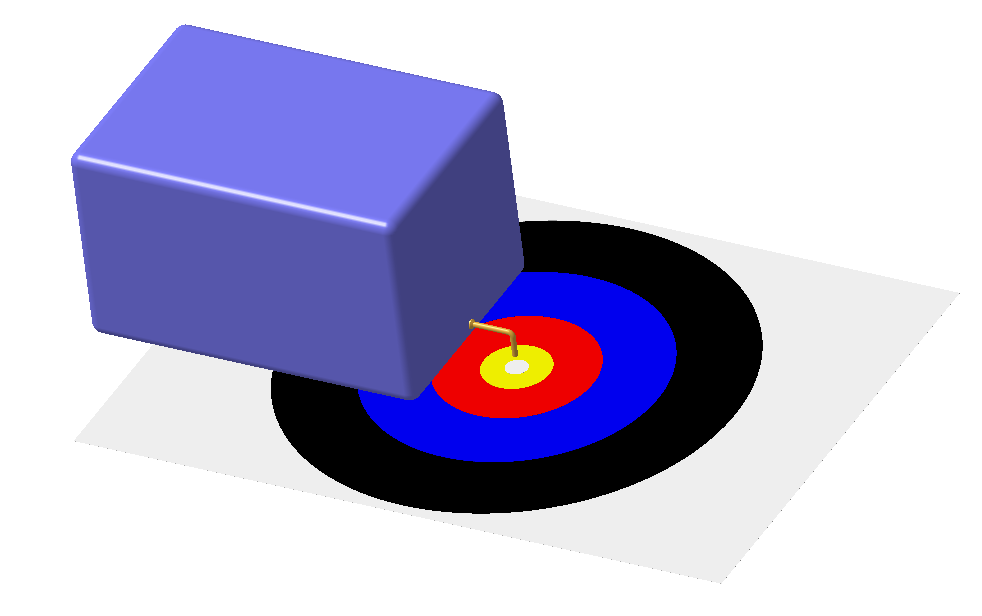
\includegraphics[width=0.7\textwidth]{extracted_images/image_10_2.png}
\end{center}\vspace{0.6em}\noindent
As you can see from the picture provided of the car, you can see that we have fully manufactured a working car that follows all the guidelines and specifications that were required. The main aim of this competition was to create a device that could reach a target there and back under three minutes. The datum pointer should start in the centre of the target and move towards the wall. It should then touch the end of the wall and stay there for 15 seconds then return to the same position as before where the datum pointer started from. The device was safe to use since we ensures that all rules were carefully followed such as electrical connections not being exposed or having the car not fit within the maximum envelope.\\[1em]
As you can see, we received no penalties given since our datum pointer was not too high from the ground. Our front plunger was not larger that it was allowed, and it could realign between the two vertical targets. If the above was not completed it would have resulted in penalties for our team.\\[1em]
The size of envelope is 400x400x400mm which our device was within regulation of. The device should also be able to fit within the envelope throughout the whole competition. We ensured that the datum pointer is in a vertical position and is pointing downwards.

\newpage
\section{References}

\end{document}